\textbf{Phần 1. Trắc nghiệm lựa chọn (Học sinh quan sát sơ đồ và chọn đáp án đúng)}
\setcounterpageref{ex}{0}

% --- CÂU 1 ---
\begin{ex} %[1D1N05]
Quan sát sơ đồ tách số: Số $3$ gồm $1$ và mấy?
\begin{center}
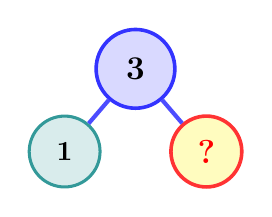
\begin{tikzpicture}[scale=0.75, baseline=(current bounding box.center)]
  \node[draw=blue!80, fill=blue!15, circle, line width=1.3pt, minimum size=1cm, font=\large\bfseries] (T) at (0,1.2) {3};
  \node[draw=teal!80, fill=teal!15, circle, line width=1.1pt, minimum size=0.9cm, font=\bfseries] (L) at (-1.2,-0.2) {1};
  \node[draw=red!80, fill=yellow!25, circle, line width=1.3pt, minimum size=0.9cm, font=\large\bfseries, text=red] (R) at (1.2,-0.2) {?};
  \draw[line width=1.5pt, blue!70] (T) -- (L);
  \draw[line width=1.5pt, blue!70] (T) -- (R);
\end{tikzpicture}
\end{center}
\choice
{\True $2$}
{$1$}
{$3$}
{$4$}
\loigiai{
Tách số: $3$ gồm $1$ và $2$.\\
\textbf{Đáp án của câu hỏi là A}
}
\end{ex}

% --- CÂU 2 ---
\begin{ex} %[1D1N05]
Quan sát sơ đồ tách số: Số $4$ gồm $2$ và mấy?
\begin{center}
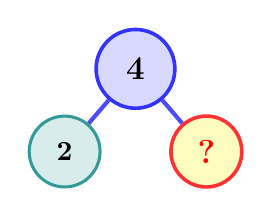
\begin{tikzpicture}[scale=0.75, baseline=(current bounding box.center)]
  \node[draw=blue!80, fill=blue!15, circle, line width=1.3pt, minimum size=1cm, font=\large\bfseries] (T) at (0,1.2) {4};
  \node[draw=teal!80, fill=teal!15, circle, line width=1.1pt, minimum size=0.9cm, font=\bfseries] (L) at (-1.2,-0.2) {2};
  \node[draw=red!80, fill=yellow!25, circle, line width=1.3pt, minimum size=0.9cm, font=\large\bfseries, text=red] (R) at (1.2,-0.2) {?};
  \draw[line width=1.5pt, blue!70] (T) -- (L);
  \draw[line width=1.5pt, blue!70] (T) -- (R);
\end{tikzpicture}
\end{center}
\choice
{$1$}
{\True $2$}
{$3$}
{$4$}
\loigiai{
Tách số: $4$ gồm $2$ và $2$.\\
\textbf{Đáp án của câu hỏi là B}
}
\end{ex}

% --- CÂU 3 ---
\begin{ex} %[1D1H05]
Quan sát sơ đồ gộp số: Gộp $2$ và $3$ được mấy?
\begin{center}
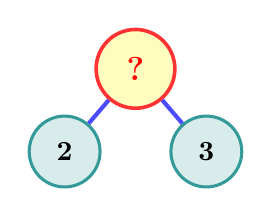
\begin{tikzpicture}[scale=0.75, baseline=(current bounding box.center)]
  \node[draw=red!80, fill=yellow!25, circle, line width=1.3pt, minimum size=1cm, font=\large\bfseries, text=red] (T) at (0,1.2) {?};
  \node[draw=teal!80, fill=teal!15, circle, line width=1.1pt, minimum size=0.9cm, font=\bfseries] (L) at (-1.2,-0.2) {2};
  \node[draw=teal!80, fill=teal!15, circle, line width=1.1pt, minimum size=0.9cm, font=\bfseries] (R) at (1.2,-0.2) {3};
  \draw[line width=1.5pt, blue!70] (T) -- (L);
  \draw[line width=1.5pt, blue!70] (T) -- (R);
\end{tikzpicture}
\end{center}
\choice
{$4$}
{$6$}
{$7$}
{\True $5$}
\loigiai{
Gộp $2$ và $3$ được $5$.\\
\textbf{Đáp án của câu hỏi là D}
}
\end{ex}

% --- CÂU 4 ---
\begin{ex} %[1D1H05]
Số $5$ gồm $4$ và mấy?
\begin{center}
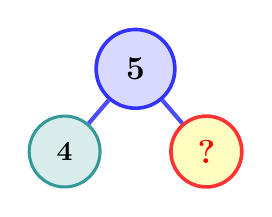
\begin{tikzpicture}[scale=0.75, baseline=(current bounding box.center)]
  \node[draw=blue!80, fill=blue!15, circle, line width=1.3pt, minimum size=1cm, font=\large\bfseries] (T) at (0,1.2) {5};
  \node[draw=teal!80, fill=teal!15, circle, line width=1.1pt, minimum size=0.9cm, font=\bfseries] (L) at (-1.2,-0.2) {4};
  \node[draw=red!80, fill=yellow!25, circle, line width=1.3pt, minimum size=0.9cm, font=\large\bfseries, text=red] (R) at (1.2,-0.2) {?};
  \draw[line width=1.5pt, blue!70] (T) -- (L);
  \draw[line width=1.5pt, blue!70] (T) -- (R);
\end{tikzpicture}
\end{center}
\choice
{\True $1$}
{$0$}
{$2$}
{$3$}
\loigiai{
$5$ gồm $4$ và $1$.\\
\textbf{Đáp án của câu hỏi là A}
}
\end{ex}

% --- CÂU 5 ---
\begin{ex} %[1D1H05]
Gộp $3$ và $3$ được mấy?
\begin{center}
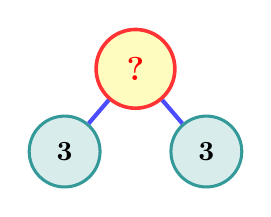
\begin{tikzpicture}[scale=0.75, baseline=(current bounding box.center)]
  \node[draw=red!80, fill=yellow!25, circle, line width=1.3pt, minimum size=1cm, font=\large\bfseries, text=red] (T) at (0,1.2) {?};
  \node[draw=teal!80, fill=teal!15, circle, line width=1.1pt, minimum size=0.9cm, font=\bfseries] (L) at (-1.2,-0.2) {3};
  \node[draw=teal!80, fill=teal!15, circle, line width=1.1pt, minimum size=0.9cm, font=\bfseries] (R) at (1.2,-0.2) {3};
  \draw[line width=1.5pt, blue!70] (T) -- (L);
  \draw[line width=1.5pt, blue!70] (T) -- (R);
\end{tikzpicture}
\end{center}
\choice
{$5$}
{$7$}
{\True $6$}
{$8$}
\loigiai{
Gộp $3$ và $3$ được $6$.\\
\textbf{Đáp án của câu hỏi là C}
}
\end{ex}

% --- CÂU 6 ---
\begin{ex} %[1D1H05]
Số $6$ gồm $5$ và mấy?
\begin{center}
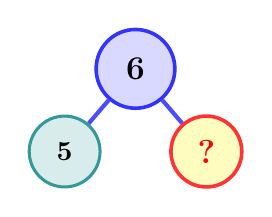
\begin{tikzpicture}[scale=0.75, baseline=(current bounding box.center)]
  \node[draw=blue!80, fill=blue!15, circle, line width=1.3pt, minimum size=1cm, font=\large\bfseries] (T) at (0,1.2) {6};
  \node[draw=teal!80, fill=teal!15, circle, line width=1.1pt, minimum size=0.9cm, font=\bfseries] (L) at (-1.2,-0.2) {5};
  \node[draw=red!80, fill=yellow!25, circle, line width=1.3pt, minimum size=0.9cm, font=\large\bfseries, text=red] (R) at (1.2,-0.2) {?};
  \draw[line width=1.5pt, blue!70] (T) -- (L);
  \draw[line width=1.5pt, blue!70] (T) -- (R);
\end{tikzpicture}
\end{center}
\choice
{$2$}
{$3$}
{\True $1$}
{$4$}
\loigiai{
$6$ gồm $5$ và $1$.\\
\textbf{Đáp án của câu hỏi là C}
}
\end{ex}

% --- CÂU 7 ---
\begin{ex} %[1D1V05]
Gộp $4$ và $4$ được mấy?
\begin{center}
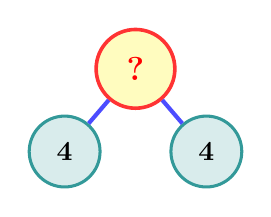
\begin{tikzpicture}[scale=0.75, baseline=(current bounding box.center)]
  \node[draw=red!80, fill=yellow!25, circle, line width=1.3pt, minimum size=1cm, font=\large\bfseries, text=red] (T) at (0,1.2) {?};
  \node[draw=teal!80, fill=teal!15, circle, line width=1.1pt, minimum size=0.9cm, font=\bfseries] (L) at (-1.2,-0.2) {4};
  \node[draw=teal!80, fill=teal!15, circle, line width=1.1pt, minimum size=0.9cm, font=\bfseries] (R) at (1.2,-0.2) {4};
  \draw[line width=1.5pt, blue!70] (T) -- (L);
  \draw[line width=1.5pt, blue!70] (T) -- (R);
\end{tikzpicture}
\end{center}
\choice
{$7$}
{\True $8$}
{$9$}
{$10$}
\loigiai{
Gộp $4$ và $4$ được $8$.\\
\textbf{Đáp án của câu hỏi là B}
}
\end{ex}

% --- CÂU 8 ---
\begin{ex} %[1D1V05]
Số $7$ gồm $3$ và mấy?
\begin{center}
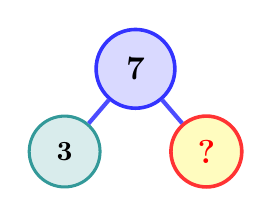
\begin{tikzpicture}[scale=0.75, baseline=(current bounding box.center)]
  \node[draw=blue!80, fill=blue!15, circle, line width=1.3pt, minimum size=1cm, font=\large\bfseries] (T) at (0,1.2) {7};
  \node[draw=teal!80, fill=teal!15, circle, line width=1.1pt, minimum size=0.9cm, font=\bfseries] (L) at (-1.2,-0.2) {3};
  \node[draw=red!80, fill=yellow!25, circle, line width=1.3pt, minimum size=0.9cm, font=\large\bfseries, text=red] (R) at (1.2,-0.2) {?};
  \draw[line width=1.5pt, blue!70] (T) -- (L);
  \draw[line width=1.5pt, blue!70] (T) -- (R);
\end{tikzpicture}
\end{center}
\choice
{\True $4$}
{$3$}
{$5$}
{$2$}
\loigiai{
$7$ gồm $3$ và $4$.\\
\textbf{Đáp án của câu hỏi là A}
}
\end{ex}

% --- CÂU 9 ---
\begin{ex} %[1D1V05]
Gộp $5$ và $5$ được mấy?
\begin{center}
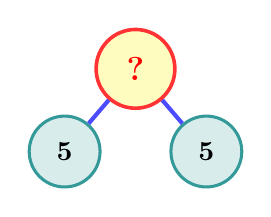
\begin{tikzpicture}[scale=0.75, baseline=(current bounding box.center)]
  \node[draw=red!80, fill=yellow!25, circle, line width=1.3pt, minimum size=1cm, font=\large\bfseries, text=red] (T) at (0,1.2) {?};
  \node[draw=teal!80, fill=teal!15, circle, line width=1.1pt, minimum size=0.9cm, font=\bfseries] (L) at (-1.2,-0.2) {5};
  \node[draw=teal!80, fill=teal!15, circle, line width=1.1pt, minimum size=0.9cm, font=\bfseries] (R) at (1.2,-0.2) {5};
  \draw[line width=1.5pt, blue!70] (T) -- (L);
  \draw[line width=1.5pt, blue!70] (T) -- (R);
\end{tikzpicture}
\end{center}
\choice
{$9$}
{$8$}
{$7$}
{\True $10$}
\loigiai{
Gộp $5$ và $5$ được $10$.\\
\textbf{Đáp án của câu hỏi là D}
}
\end{ex}

% --- CÂU 10 ---
\begin{ex} %[1D1V05]
Số $8$ gồm $5$ và mấy?
\begin{center}
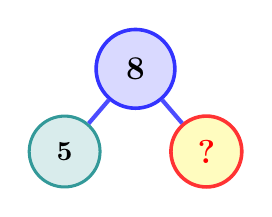
\begin{tikzpicture}[scale=0.75, baseline=(current bounding box.center)]
  \node[draw=blue!80, fill=blue!15, circle, line width=1.3pt, minimum size=1cm, font=\large\bfseries] (T) at (0,1.2) {8};
  \node[draw=teal!80, fill=teal!15, circle, line width=1.1pt, minimum size=0.9cm, font=\bfseries] (L) at (-1.2,-0.2) {5};
  \node[draw=red!80, fill=yellow!25, circle, line width=1.3pt, minimum size=0.9cm, font=\large\bfseries, text=red] (R) at (1.2,-0.2) {?};
  \draw[line width=1.5pt, blue!70] (T) -- (L);
  \draw[line width=1.5pt, blue!70] (T) -- (R);
\end{tikzpicture}
\end{center}
\choice
{$2$}
{$4$}
{$5$}
{\True $3$}
\loigiai{
$8$ gồm $5$ và $3$.\\
\textbf{Đáp án của câu hỏi là D}
}
\end{ex}

% --- CÂU 11 ---
\begin{ex} %[1D1V05]
Gộp $6$ và $3$ được mấy?
\begin{center}
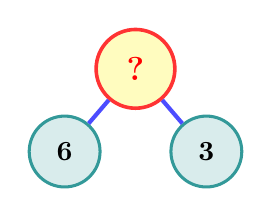
\begin{tikzpicture}[scale=0.75, baseline=(current bounding box.center)]
  \node[draw=red!80, fill=yellow!25, circle, line width=1.3pt, minimum size=1cm, font=\large\bfseries, text=red] (T) at (0,1.2) {?};
  \node[draw=teal!80, fill=teal!15, circle, line width=1.1pt, minimum size=0.9cm, font=\bfseries] (L) at (-1.2,-0.2) {6};
  \node[draw=teal!80, fill=teal!15, circle, line width=1.1pt, minimum size=0.9cm, font=\bfseries] (R) at (1.2,-0.2) {3};
  \draw[line width=1.5pt, blue!70] (T) -- (L);
  \draw[line width=1.5pt, blue!70] (T) -- (R);
\end{tikzpicture}
\end{center}
\choice
{$8$}
{$10$}
{\True $9$}
{$7$}
\loigiai{
Gộp $6$ và $3$ được $9$.\\
\textbf{Đáp án của câu hỏi là C}
}
\end{ex}

% --- CÂU 12 ---
\begin{ex} %[1D1C05]
Số $10$ gồm $6$ và mấy?
\begin{center}
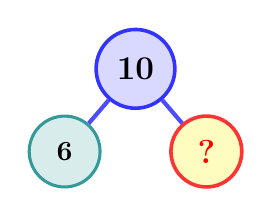
\begin{tikzpicture}[scale=0.75, baseline=(current bounding box.center)]
  \node[draw=blue!80, fill=blue!15, circle, line width=1.3pt, minimum size=1cm, font=\large\bfseries] (T) at (0,1.2) {10};
  \node[draw=teal!80, fill=teal!15, circle, line width=1.1pt, minimum size=0.9cm, font=\bfseries] (L) at (-1.2,-0.2) {6};
  \node[draw=red!80, fill=yellow!25, circle, line width=1.3pt, minimum size=0.9cm, font=\large\bfseries, text=red] (R) at (1.2,-0.2) {?};
  \draw[line width=1.5pt, blue!70] (T) -- (L);
  \draw[line width=1.5pt, blue!70] (T) -- (R);
\end{tikzpicture}
\end{center}
\choice
{$3$}
{\True $4$}
{$5$}
{$6$}
\loigiai{
$10$ gồm $6$ và $4$.\\
\textbf{Đáp án của câu hỏi là B}
}
\end{ex}

% =========================================================================
% PHẦN 2: TRẮC NGHIỆM ĐÚNG SAI (QUAN SÁT TRANH MINH HỌA)
% =========================================================================
\textbf{Phần 2. Trắc nghiệm đúng sai (Xét tính đúng/sai của các sơ đồ)}
\setcounterpageref{ex}{0}

% --- CÂU 13 ---
\begin{ex} %[1D1H05]
Xét tính đúng sai của các cách tách gộp số dưới đây:
\choiceTF
{\True Số $5$ gồm $2$ và $3$.}
{\True Gộp $4$ và $2$ được $6$.}
{Số $7$ gồm $5$ và $3$.}
{\True Gộp $1$ và $6$ được $7$.}
\loigiai{
\begin{itemize}
    \item $5$ gồm $2$ và $3$: \textbf{Đúng}.
    \item Gộp $4$ và $2$ được $6$: \textbf{Đúng}.
    \item $7$ gồm $5$ và $2$ (nói $3$ là sai): \textbf{Sai}.
    \item Gộp $1$ và $6$ được $7$: \textbf{Đúng}.
\end{itemize}
}
\end{ex}

% --- CÂU 14 ---
\begin{ex} %[1D1V05]
Xét các cách tách số $8$ thành hai phần:
\choiceTF
{\True Số $8$ gồm $4$ và $4$.}
{\True Số $8$ gồm $5$ và $3$.}
{Số $8$ gồm $6$ và $1$.}
{\True Số $8$ gồm $7$ và $1$.}
\loigiai{
\begin{itemize}
    \item $8$ gồm $4$ và $4$: \textbf{Đúng}.
    \item $8$ gồm $5$ và $3$: \textbf{Đúng}.
    \item $8$ gồm $6$ và $2$ (nói $1$ là sai): \textbf{Sai}.
    \item $8$ gồm $7$ và $1$: \textbf{Đúng}.
\end{itemize}
}
\end{ex}

% =========================================================================
% PHẦN 3: TRẢ LỜI NGẮN (ĐIỀN SỐ THÍCH HỢP VÀO Ô TRỐNG)
% =========================================================================
\textbf{Phần 3. Trả lời ngắn (Quan sát sơ đồ và điền số thích hợp)}
\setcounterpageref{ex}{0}

% --- CÂU 15 ---
\begin{ex} %[1D1H05]
Số $4$ gồm $1$ và mấy?
\shortans{3}
\loigiai{
\textbf{Đáp số:} $3$\\
$4$ gồm $1$ và $3$.
}
\end{ex}

% --- CÂU 16 ---
\begin{ex} %[1D1H05]
Gộp $3$ và $4$ được mấy?
\shortans{7}
\loigiai{
\textbf{Đáp số:} $7$\\
Gộp $3$ và $4$ được $7$.
}
\end{ex}

% --- CÂU 17 ---
\begin{ex} %[1D1V05]
Số $9$ gồm $7$ và mấy?
\shortans{2}
\loigiai{
\textbf{Đáp số:} $2$\\
$9$ gồm $7$ và $2$.
}
\end{ex}

% --- CÂU 18 ---
\begin{ex} %[1D1V05]
Gộp $2$ và $6$ được mấy?
\shortans{8}
\loigiai{
\textbf{Đáp số:} $8$\\
Gộp $2$ và $6$ được $8$.
}
\end{ex}

% --- CÂU 19 ---
\begin{ex} %[1D1V05]
Số $10$ gồm $8$ và mấy?
\shortans{2}
\loigiai{
\textbf{Đáp số:} $2$\\
$10$ gồm $8$ và $2$.
}
\end{ex}

% --- CÂU 20 ---
\begin{ex} %[1D1C05]
Gộp $5$ và $4$ được mấy?
\shortans{9}
\loigiai{
\textbf{Đáp số:} $9$\\
Gộp $5$ và $4$ được $9$.
}
\end{ex}
